%
\chapter{Image Quality Assessment}
%
In this section we attempt to estimate the overall \textit{watchability} of the footage we have in our dataset. This forms the basis for knowing which parts of the videos are suitable for human observation in a final video summary.
%
\section{Literature study}
%
Girgensohn et al.\cite{Girgensohn:2000:SAH:354401.354415} describes a method to estimate the camera motion in a video by computing a shift-vector between subsequent frames. They also look into lighting conditions in individual frames by calculating the percentage of pixels within a specific boundary; an indication of reasonable exposure levels in the frame.\\
The \textit{spring loading effect}\cite{Girgensohn:2000:SAH:354401.354415}, also described by Girgensohn et al., is a way to balance clip lengths. Each frame is given an \textit{unsuitability} score based on the image quality in the frame, and the camera motion in the area around the frame. It treats the \textit{unsuitability} of the surrounding frames as an additional cost for including them in the clip. The purpose of this is to automatically fit segmented clips to match a desired total clip length.\\
A more comprehensive approach described by Wu et al.\cite{10.1109/ICME.2005.1521399} is a multi-level classifier that labels each frame as belonging to one of the groups: \textit{blurred}, \textit{shaky}, \textit{inconsistent} and \textit{stable}. Their solution yield satisfactory results, but does rely on the training a Support Vector Machine.
%
\section{Method}
%
We define suitable footage to mean video segments, which are not too shaky or fast panning to be considered watchable. As a rule of thumb, a human observer should be able to watch the videos without being annoyed by the movement of the camera. Further more, we want the content in the video to be clearly visible. Footage, which is too dark or bright, or depict textureless surfaces should be discarded.
%
\subsection{Frame Shift Estimation}\label{sec:frame_shift_estimation}
%
We estimate the magnitude of the shift of content between neighbouring frames, and use it as an indication of the \textit{egomotion} (camera movement).\\
Girgensohn et al.\cite{Girgensohn:2000:SAH:354401.354415} estimates the shift in two subsequent frames, where the direction of a vector is the direction of the shift of content, and the magnitude of that vector how many pixels it was shifted. We choose this method due to its implementational simplicity and low computational costs.\\
For each pair of subsequent frames, the latter frame is shifted around, in all four directions (up, down, left, right). The initial shift distance is 32 pixels (suggested by Girgensohn et al.). In each iteration this distance is halved. 
% For each direction, in each iteration 
With each shift the Root-Mean-Square (\textit{RMS}) of the difference between the shifted frame and the previous unshifted frame is calculated. The direction with the lowest \textit{RMS} is the basis for the following iteration.
%
If $v \in V$ is a vector representing a selected shift in an iteration, then $V$ is the set of all shifts performed over all iterations. The shift vector magnitude estimating the intensity of camera motion between two frames is then defined as:
%
\[
s = \|\sum V\|
\]
%
The \textit{shift vector magnitude ratio}, $S$, is defined as:
%
\[
S = s^2 / M^2, 
\]
%
where $M$ is the largest possible magnitude of the shift vector. A shift in the same direction in each iteration of the shift vector computation will in our configuration at most shift $32+16+8+4+2+1=63$ pixels. We square $s$ and $M$ in order to increase the sensitivity toward bad frames, while still keeping $S$ normalized to [0,1].\\
%
At 24 frames per second (fps) this method can theoretically trace camera movements of up to $24 \times (32+16+8+4+2+1) = 1512$ pixels per second, in any direction. I.e. for frames with a resolution of $\sim$ $640\times360$, even extremely fast camera motion should, in at least in theory, be detected (accuracy is here highly dependant on the blurriness of the frames).
%
\subsection{Frame Contrast Estimation}\label{sec:frame_contrast_estimation}
%
Girgensohn et al.\cite{Girgensohn:2000:SAH:354401.354415} also describes a method of determining the level of brightness in the image by computing the fraction of pixels above a certain brightness threshold. While this is a sufficient measure for detecting dark images, it does not detect very bright ones, nor images dominated by textureless surfaces. Our method does not have this disadvantage as we compute a measure of contrast as $c = std(X)$, where $X$ is the image matrix.\\
A small standard deviation indicates little contrast/diversity in pixel intensity, ie. a overly dark/bright image, or an image with little texture, which makes features in the image hard to distinguish. A high standard deviation indicates a high contrast/much diversity in pixel intensity, ie. a textured image or an image with a high variation of pixel intensity which makes features in the image easy to distinguish.\\
%
The \textit{contrast} ratio, $C$, is defined as:
\[
C = 1 - c^2 / N^2,
\]
where $N$ is the largest possible value of $c$. Again, we square both $c$ and $N$ to increase sensitivity toward bad frames. For our 8-bit grayscale footage $N = 127.5$, which would be the standard deviation for a frame, whos image-matrix contain only values of 0 and 255, uniformly distributed. We subtract the ratio from 1 in order to make it comparable to the shift vector magnitude ratio.\\
%
\subsection{Triangular Smoothing}\label{sec:triangularsmoothing}
%
Both $S$ and $C$ are meassures of how unsuitable a frame is. We perform \textit{trianglur smoothing} on the set of all $S$ and $C$ over all frames in a video, in order to remove outliers which can lead to a misclassification. Triangular smoothing is a weighted smoothing function where the degree of smoothing determines the distribution of weights. The largest weight, $w_0$, is given to the element we wish to smooth. %The weight of the elements surrounding it 
The other weights are determined by their distance to $w_0$, and decrease in a linear fashion. We define the weight function, $T(w)$, as:
%
\begin{equation}
T(w) = [1,2,\dots,w-1,w,w+1,\dots,2,1].
\end{equation}\label{eq:triangular}
%
% where $w$ is the weight of the element we want to smooth.
Triangular smoothing can then be described by:
%
\[
S(x, w) = \sum_{i=x-w}^{x+w} \frac{D_{i} T(w)_{i-(x-w)}}{\sum T(w)},
\]
%
where $x$ is the index of the element we wish to smooth, $w$ is the applied weight, and $D$ is the set of all original values. %, and $T$ is the triangle of weights defined in \ref{eq:triangular}. 
KAN VI LIIIIIGE FÅR DEN HER FORMULERET?
For simplicity we have excluded the border cases at the beginning and the end of $D$, where $T(w)$ covers values that are not defined. In those cases we simply calculate $S$ and $T$ for the values, which \textit{are} defined. Figure \ref{fig:triangularsmoothing} shows the result of performing triangular smoothing on a collection of data, with various values of $w$. We fix $w = 12$ which roughly represents 1 second of footage.
%
\begin{figure}
     \centering
     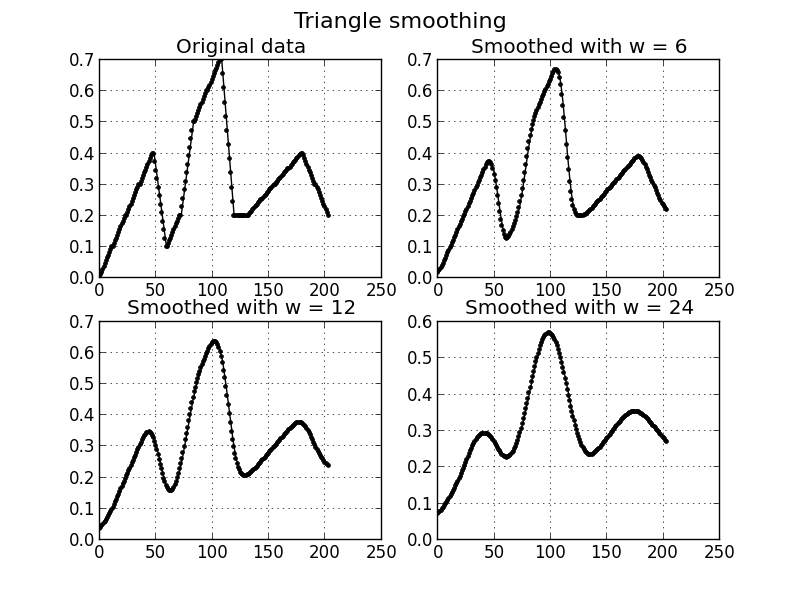
\includegraphics[width=1\textwidth]{img/triangle_smooth.png}
     \caption{An example of triangular smoothing being applied to arbitary data for various values of $w$.}
     \label{fig:triangularsmoothing}
\end{figure}
%
\subsection{Frame State Classification}
%
The classifiers described in section \ref{sec:algorithms} takes the the shift vector magnitude ratios and contrast ratios, for a video, and calculate a unsuitability measure, $v$, for each frame. This unsuitability meassure is then used to perform a binary classification of each frame as being either \textit{good} or \textit{bad}. Unless otherwise noted, this classification is defined as:
\begin{equation}
s = 
\begin{cases}
\text{good} & \text{ if } v \leq 1\\
\text{bad} & \text{ otherwise }
\end{cases}
\end{equation}\label{equ:frame_state_classif}
%
\subsection{Classifiers}\label{sec:algorithms}
%
We have developed 4 different classifiers, each taking a different approach as described in the following.
%
\subsubsection{Contrast Only classification (CO)}
%
This classifier focuses on the contrast ratios throughout a video. The frame unsutability meassure, $v$, is defined as $v=\frac{C}{\tau}$, where $\tau$ is some treshold and $C$ is the contrast ratio for that frame.
%
\subsubsection{Shift Magnitude Only classification (SO}
%
This classifier focuses on the shift vector magnitude ratios for each frame. The frame unsutability meassure, $v$, is defined as $v=\frac{S}{\tau}$, where $\tau$ is some treshold and $S$ is the shift vector magnitude ratio for that frame.
%
\subsubsection{Independent Contrast and Shift Magnitude classification (ICSM)}
%
This methods ignores the cumulative effect of the contrast and shift vector magnitude ratio, and is similar to the approach taken by Girgensohn et al.\cite{Girgensohn:2000:SAH:354401.354415}. We look at the contrast ratio and the shift vector magnitude ratios independantly and classifies frames as described in (\ref{equ:frame_state_classif}). The frame unsutability meassure, $v$, is defined as $v=\text{max}(\frac{C}{\tau_1}, \frac{S}{\tau_2})$, where $C$ is the contrast ratio, $S$ is the shift vector magnitude ratio, and $\tau_1$ and $\tau_2$ are some tresholds.
%
\subsubsection{Cummulative Contrast and Shift Magnitude classification (CCSM)}
%
This method investigates the cumulative effect of both ratios. If a weighed sum of the two ratios exceeds a certain threshold, the frame is classified as \textit{bad}. In this particular case the frame state is defined as follows:\\
%
\[
s = 
\begin{cases}
\text{good} & \text{ if } v \leq \tau\\
\text{bad} & \text{ otherwise }
\end{cases},
\]
%
where the frame unsutability measure is defined as $v=(1-w) C + w S$, where $C$ is the contrast ratio, $S$ is the shift vector magnitude ratio, $\tau$ is a threshold and $w$ is a weighing between the two ratios.
%
\section{Dataset}
%
This section describe details about our dataset that are only relevant for image quality assesment. We categorize the videos YouTube videos as being either unedited or pre-edited. The former is the most desireable as this is presumeably raw footage.
%
\subsection{Unedited YouTube Videos}
%
The dataset contains 25 raw videos. The length of the clips range from 10 seconds to 10 minutes, totaling somewhere around one hour of footage. All videos appear to have been recorded using hand-held devices so the quality of the footage varies a lot. In order to be able to train and test on this part of the dataset, we generate a \textit{gold standard} manually for each video as descibed in section \ref{sec:goldstandard} below.
%
\subsection{Pre-edited YouTube videos}
%
Most videos available on YouTube have already been edited in some way. Our dataset contain 16 pre-edited vidoes ($\sim$ 30 minutes). In order to use this footage we cut each video into multiple clips, at the points of its scene boundaries. This editing is done manually. Because some of these scenes are undesireable we also perform a manual clean up. Examples of scenes which are removed are; scenes with much on-screen text, credits, montages, ie. scenes that would not be considered raw footage, as well as very short scenes. Footage, which has undergone editing such as \textit{frame stabilisation}, are slowed down, or sped up, are not removed.
%
\subsection{Own recordings}
%
The dataset also contains five videos, which we have recorded ourselves. These videos depict various scenarios involving low contrast and darkness, shakiness, fast camera movement and completely still footage. These videos serve as a starting point for parameter tuning. Unlike much of the other footage, which is also used throughout the later phases, these videos are only used in our image quality assesement experiments.
%
%
\subsection{Gold Standard}\label{sec:goldstandard}
%
In order to be able to test the performance of our classifiers we genererate a \textit{gold standard} for each video. For the unedited YouTube videos and our own recordings, this is done by manually marking all frames as being either \textit{good} or \textit{bad}.\\
Since the pre-edited youtube videos have already undergone a manual screening and editing process, we assume all their frames to be \textit{good}.\\
These gold standards are used as the absolute truth, when we meassure the performance of our classifiers.
%
\section{Findings}
%
Due to the limited size of our data we perform a \emph{k-fold cross validation}, as described in section \ref{sec:kfoldxval}, during our tests. The metric of success is whether a method correctly estimates the state of the frames, in respect to the \text{gold standard}. We investigate both the performance of the various classifiers, and also their robustness as a measure of how sensitive they are to parameter change.\\
For each classifier we determine the optimal configuration of parameter(s), over $k$ iterations, and calculate a mean based on our findings. The robustness, which is estimated as a function of how well the classifier performs over all tested configurations, is calculated on the entire dataset. We also record some of the side-effects of each configuration such as the average length of a good and bad sequences.\\
%
\subsection{K-fold Cross Validation}\label{sec:kfoldxval}
%
 In k-fold cross validation the dataset is randomly partitioned into $k$ subsets of which one is retained for testing the method and the remaining $k-1$ subsets are used for training. The cross validation is repeated $k$ times, each time using a different subsets for testing. The resulting score and parameter(s) from each fold is usually averaged.
%
\subsection{Parameter tuning}\label{sec:ph1tweaking}
%
Parameter tuning is often a matter of maximising positive \textit{precision} and \textit{recall}. Positive precision is the certainty with which we can say that a positive classification is correct:
\[
\text{Positive Precision } = \frac{\text{\#true positives}}{\text{\#true positives + \#false positives}},
\]
whereas positive recall is the ratio of true positives found compared to how many actually exists:
\[
\text{Positive Recal } = \frac{\text{\#true positives}}{\text{\#true positives + \#false negatives}}.
\]
% Our approach is a little different. Because 
As our dataset contain mostly \textit{good} frames we instead wish to award a classifier that detect the few \textit{bad} frames that \textit{are} present. We therfore attempt to maximise positive precision along with \textit{negative} recall.\\
In order to quantify the quality of our choice of parameter(s) we look at the benefit we gain from it versus the cost that we pay. We define the cost, \textit{C} as:
%
\[
C = 1 - 2\frac{P_{r}N_{p}}{P_{r} + N_{p}},
\]
%
and the benefit, \text{B}, as:
%
\[
B = 2\frac{N_{r} P_{p}}{N_{r} + P_{p}},
\]
%
where $P_r$ is positive recall, $N_p$ is negative precision, $P_r$ is positive recall, and $N_p$ is negative precision. In each case we combine the two factors we want to meassure by calculating their evenly distributed harmonic mean. FORMULER? We can then plot $C$ and $B$, for various parameter choices, in a diagram and use this a tool for comparing different configurations of a classifier. Figure \ref{fig:costbenefitdiagram} shows an example of such a diagram.
%
\begin{figure}
     \centering
     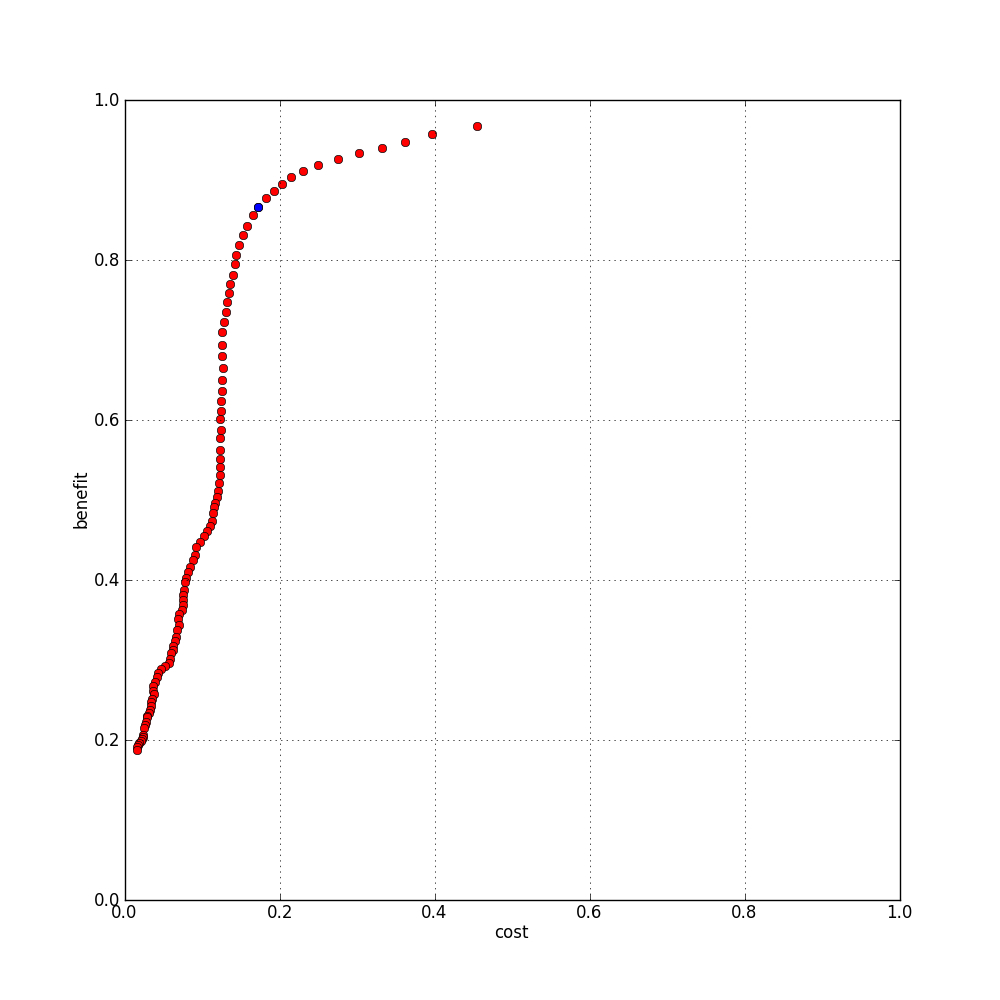
\includegraphics[width=0.75\textwidth]{img/2dcostbenefitexample2.jpg}
     \caption{An example of a classifier cost/benefit diagram for various parameter selections, the blue point represents the best configuration}
     \label{fig:costbenefitdiagram}
\end{figure}
%
In order to determine the best configuration we calculate the distance from each point to the (1,0) coordinate in the diagram. Since this coordinate represents the best possible performance (maximum benefit, with no cost) we argue that the distance score is reasonable way to compare the performance of different configurations.\footnote{We have later realised that this method has some drawbacks. We have come up with a different way to meassure performance which is described in our Discussion section for this chapter \ref{sec:phase1discussion}.}\\
%
\subsection{Robustness}\label{sec:robustness}
%
On top of the ordinary parameter tuning and testing, we also attempt to measure the overall robustness of each of the classifiers, with respect to changes of parameters.\\
Relative Operating Characteristics (\textit{ROC}) diagrams, as described by Fawcett\cite{Fawcett06a}, are a useful tool for quantifying the overall stability of an algorithm. The ROC diagrams plot different parameter configurations as the relation between the resulting \textit{true positive rates} (the benefit) and \textit{false positive rates} (the cost). Plotting this relation yields a curve, whos underlying area can be used as an estimate of the algorithms stability, where a large area indicates a stable algorithm, and a small area indicates an unstable algorithm.\\
\\
Inspired by ROC diagrams we perform another parameter analysis for each classifier, this time using the entire dataset. We then plot the results in cost/benefit diagrams as described in section \ref{sec:ph1tweaking} and calcuate the area under the curve (\textit{AUC}) formed by the points. The larger the AUC is the more robust the classifier is toward changes to its parameter(s). Since the points produced by most of the classifiers are not evenly distributed over the x-axis of the diagram, we insert points at the (0,0) and (1,1) coordinate in order to cover the entire span. It has the effect of normalising undefined regions around $y=x$, which makes it easier to compare the AUCs across all classifiers.\\
Unlike the parameter tuning described in section \ref{sec:ph1tweaking}, we learn nothing about how the performance of the individual configurations will generalise. Instead we gain an indication of the overall ability, for each algorithm, to the perform the classification.
%
\subsection{Multi-parameter algorithms}\label{sec:ph1multiparameter}
%
All our algorithms, except one, have a single parameter. This makes the tasks of parameter tuning, and generation of cost/benefit diagrams, straightforward. The \textit{ICSM} algorithm has two parameters. The additional parameter makes parameter tuning much more computationaly expensive. All parameters in our classifiers are expressed as ratios between 0 and 1. The single-parameter classifiers are tuned by changing their single parameters by one percentage point in each iteration. This limits the number of configuration to 101. Doing the same with the \textit{ICSM} classifier would require more than 10.000 iterations, which is much too expensive.\\
In order to bring this number down we did a prelimenary probing using increments of 10 percentage point for each parameter. From the results we see that the \textit{contrast}-threshold parameter is directly corrolated with the span over which performance is defined. This is seen clearly in figure \ref{fig:3dcostbenefitdiagram}. Based on this observation, we choose to perform a full analysis where the effect of the shift vector magnitude ratio is tested down to a one percentage point precision, and the effect of the contrast ratio threshold is tested at a 10 percentage point precision.\\
This brings the total number of iterations down to $101 \times 11 = 111$.\\
\\
Another problem is that the effect of tuning more than one parameter is not illustrated very well in a two-dimensional cost/benefit diagram. The points, which really belong in a higher dimensional space, are flattened into the plane resulting in several curves without any clear connection to each other. This also makes it impossible to calcualate a meaningful AUC.\\
Instead we perform 11 analyses, one for each \textit{contrast} threshold. With one of the two parameters locked, we can perform the analysis as usual. For the parameter tuning we simply calculate the mean of the various values and parameters across all 11 analyses.\\
For the robustness test all cost/benefit curves are plottet in a three dimensional diagram where the added dimension represents the chosen contrast threshold. The plane created illustrates the robustness of the algorithm much better (see figure \ref{fig:3dcostbenefitdiagram}). Since the contrast thresholds across all iterations are uniformly distributed, we can easily determine the AUC for the algorithm by simply calculating the individual AUCs for each selection of contrast value and computing their mean.
%
\begin{figure}
     \centering
     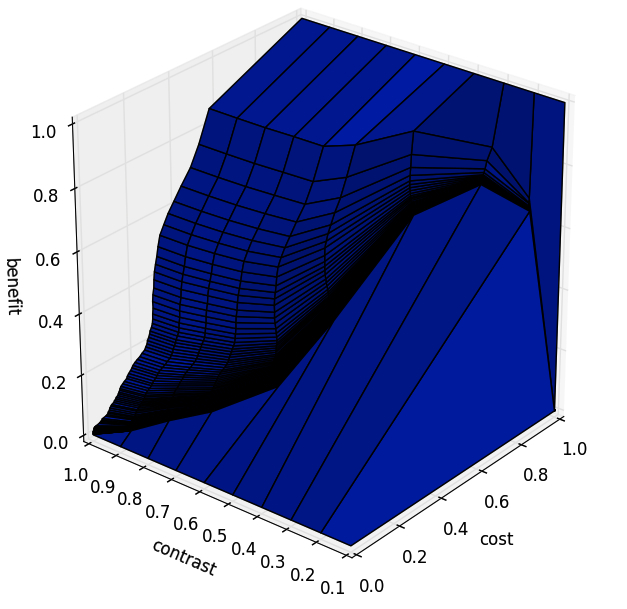
\includegraphics[width=0.75\textwidth]{img/3dcostbenefitexample.jpg}
     \caption{An example of a 3D cost/benefit diagram}
     \label{fig:3dcostbenefitdiagram}
\end{figure}
%
\subsection{Test cases}\label{sec:testcases}
%
We perform two different tests. The first (described in section \ref{sec:fbfclass}) treats all classifications equally, while the second (described in section \ref{sec:tempclass}) also looks at the at the gold standard of surrounding frames and use this information as a metric for determining how to rate misclassifications. Finally we also experiment with various degrees of smoothing of the classifier results. This is described in section \ref{sec:classsmooth}
%
\subsubsection{Frame by frame comparison (FFC)}\label{sec:fbfclass}
%
For each frame we compare the classifier results with our gold standard. We treat classifications as being either \textit{true} or \textit{false} and use the amount of true and false positives/negatives to calculate their respective precision and recall.
%
\subsubsection{Temporal comparison (TC)}\label{sec:tempclass}
%
Instead of looking at frames as individual entities we now look at the video as a whole. We treat a video as consisting of a sequence of \textit{good} and \textit{bad} segments. As we iterate through the frames of the video we change back and fourth between these two states. Misclassifications, which happen close to these change-of-state's are punished less than those that happens elsewhere. The rationale behind this is that it is difficult to objectively determine the exact point (frame) where a human observer will consider the quality of a video as changing from one state to the other. Likewise, we do not expect a human observer to notice very short segments of good- or bad- quality footage, if they are surrounded by a significant amount of footage of the opposite type.\\
For this we need a more advanced \textit{penalty function} than the binary check from describd in section \ref{sec:fbfclass}.\\
For each video, we look at our gold standard and identify all positions in its sequence of frames where there is change of state. Let $S$ be the set of all these positions, $x$ be any position in the video and $c$ be some level of tolerance for mistakes. A \emph{penalty function} for determining the ratio of punishment for a misclassification at position $x$ is then defined as:
%
\begin{displaymath}
P(x) =1 - \text{max}_{s}(e^{-\frac{(x-s)^{2}}{2c^{2}}})
\end{displaymath}
%
This function places a series of inverted gaussian bell curves at the point of every change of state. Figure \ref{fig:penaltycurve} shows an example of this. The value $c$ defines the width of the curve and thus determines how tolerant we are toward misclassifications in general. We experiment with \textit{tolerance} values of 12, 24 and 48.
%
\begin{figure}
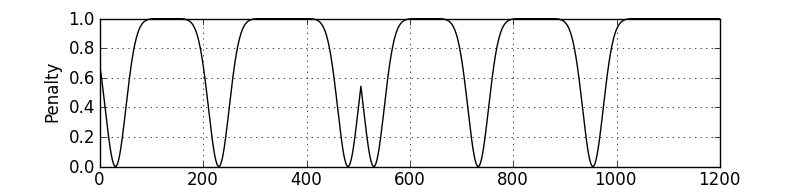
\includegraphics[width=1\textwidth]{img/penaltyfunction.jpg}
\caption{An illustration of a curve generated by the penalty function P}
\label{fig:penaltycurve}
\end{figure}
%
\emph{P(x)} always returns a ratio between 0 and 1, which tells us how severe a misclassification at position $x$ is. All correct classifications are treated just like in the FFC test case. However, if a misclassification occurs, we look at the \textit{penalty function} to see how the hard it should be punished. We add \textit{P(x)} to the \textit{false} ratio for this type of classification (positive or negative) and \textit{1 - P(X)} to the opposite type. That is, we quantify the classification as being both true and false to a varying degree determined by the \textit{penalty function}.
%
\subsubsection{Smoothing of the algorithm suggestions}\label{sec:classsmooth}
%
We also investigate the effect of performing triangular smoothing on the classification results. This is done to remove outliers in the final results and should not be confused with the smoothing of the \textit{contrast}- and \textit{shift vector}- magnitude ratios in the classifiers themselves. Since the results are binary, we round them back into ones and zeros after the smoothing.\\
As described in section \ref{sec:triangularsmoothing} the degree of smoothing is determined by a variable, $w$. We experiment with values $w=0$ and $w=12$.
%
\subsection{Results}
%
The performance results for all classifiers in each test case is presented in this section.\\
Table \ref{tab:algoconfigs} shows the different classifier configurations. \textit{Label} is the specific classifier configurations name. \textit{Algorithm} is the specific classifier. \textit{Smoothness Degree} is a measure of how much the classifier result is smoothed as described in \ref{sec:classsmooth}. \textit{Comparison Method} indicates if the algorithm result is compared using Frame-by-Frame Classification as described in section \ref{sec:fbfclass}, or using a Temporal Classification, as described in \ref{sec:tempclass}, using the stated \textit{Tolerance}. \textit{Parameter} is the best performing parameter configuration for a given classifier.\\
Classifier configuration and configuration is used interchangeably in the following.
%
\begin{table}[!ht]
  \begin{tabular}{| l | l | p{2cm} | p{2cm} | c | c | }\hline
    Label & Algorithm & Smoothness degree & Comparison method & Tolerance & Parameter(s)\\\hline
    ICSM1 & ICSM & 0 & FFC & N/A & (0.052, 0.720) \\\hline
    ICSM2 & ICSM & 12 & FFC & N/A & (0.054, 0.720) \\\hline
    ICSM3 & ICSM & 0 & TC & 24 & (0.060,0.720) \\\hline
    ICSM4 & ICSM & 0 & TC & 48 & (0.064,0.720) \\\hline
    ICSM5 & ICSM & 12 & TC & 24 & (0.058,0.720) \\\hline
    ICSM6 & ICSM & 12 & TC & 48 & (0.064, 0.720) \\\hline
    ICSM7 & ICSM & 0 & TC & 12 & (0.056, 0.720) \\\hline\hline
%
    CCSM1 & CCSM & 0 & FFC & N/A & 0.092 \\\hline
    CCSM2 & CCSM & 12 & FFC & N/A & 0.088 \\\hline
    CCSM3 & CCSM & 0 & TC & 24 & 0.100 \\\hline
    CCSM4 & CCSM & 0 & TC & 48 & 0.108 \\\hline
    CCSM5 & CCSM & 12 & TC & 24 & 0.094 \\\hline
    CCSM6 & CCSM & 12 & TC & 48 & 0.110 \\\hline
    CCSM7 & CCSM & 0 & TC & 12 & 0.098 \\\hline\hline
%
    CO1 & CO & 0 & FFC & N/A & 0.462 \\\hline
    CO2 & CO & 12 & FFC & N/A & 0.460 \\\hline
    CO3 & CO & 0 & TC & 24 & 0.466 \\\hline
    CO4 & CO & 0 & TC & 48 & 0.474 \\\hline
    CO5 & CO & 12 & TC & 24 & 0.468 \\\hline
    CO6 & CO & 12 & TC & 48 & 0.474 \\\hline
    CO7 & CO & 0 & TC & 12 & 0.466 \\\hline\hline
%
    SO1 & SO & 0 & FFC & N/A & 0.048 \\\hline
    SO2 & SO & 12 & FFC & N/A & 0.048 \\\hline
    SO3 & SO & 0 & TC & 24 & 0.056 \\\hline
    SO4 & SO & 0 & TC & 48 & 0.060 \\\hline
    SO5 & SO & 12 & TC & 24 & 0.056 \\\hline
    SO6 & SO & 12 & TC & 48 & 0.060 \\\hline
    SO7 & SO & 0 & TC & 12 & 0.054 \\\hline%\hline
%
    % $\text{CSM}^{3}1$ & $\text{CSM}^{3}$  & 0 & FFC & N/A & 0.366 \\\hline
    % $\text{CSM}^{3}2$ &$\text{CSM}^{3}$ & 12 & FFC & N/A & 0.366 \\\hline
    % $\text{CSM}^{3}3$ &$\text{CSM}^{3}$ & 0 & TC & 24 & 0.370 \\\hline
    % $\text{CSM}^{3}4$ &$\text{CSM}^{3}$ & 0 & TC & 48 & 0.388 \\\hline
    % $\text{CSM}^{3}5$ &$\text{CSM}^{3}$ & 12 & TC & 24 & 0.370 \\\hline
    % $\text{CSM}^{3}6$ &$\text{CSM}^{3}$ & 12 & TC & 48 & 0.382 \\\hline
    % $\text{CSM}^{3}7$ &$\text{CSM}^{3}$ & 0 & TC & 12 & 0.370 \\\hline
%
  \end{tabular}
\caption{Algorithm configurations}
\label{tab:algoconfigs}
\end{table}\\
%
Table \ref{tab:algoperf} shows performance of each algorithm configuration. The parameters of each configuration is an average over a 5-fold cross validation \textit{Parameter(s) std. dev. \%} is a measure of how we expect the configuration to generalize to other data, where a low relative standard deviation indicates high generalisability, and a high relative standard deviation indicates a low generalisability. \textit{DS} is the distance score, describe in section \ref{sec:ph1tweaking}, where a low score is achived if the algorithm configuration provides results close to the gold standard, and a high score is achived if the results was far from the gold standard. The distance score is an average over the 5-fold cross validation, and \textit{DS std. dev. \%} is hence a measure of how the performance of the configuration will generalise to other data. \textit{AUC} (Area Under the Curve), as described in \ref{sec:robustness}, is only indirectly related to the specific configuration, as it a result of all parameters configuratations we have tested. It gives an indication of how robust the algorithm performs.
%
\begin{table}
  %\begin{tabular}{| l | p{2.5cm} |p{2.5cm} | p{2.5cm} | c |}\hline
  \begin{tabular}{| !l | ^p{2.5cm} | ^p{2.5cm} | ^p{2.5cm} | ^c |}\hline
    Label & Parameter(s) std. dev. \% & DS & DS std. dev. \% & AUC \\\hline
    ICSM1 & (7.7\%, 5.6\%) & 0.54 & 27.17\% & 0.51 (39.44\%) \\\hline
    CCSM1 & ~4.3\% & 0.54 & 27.90\% & 0.66 \\\hline
    CO1 & ~2.5\% & 0.81 & 28.10\% & 0.40 \\\hline
    SO1 & 15.6\% & 0.55 & 27.08\% & 0.65 \\\hline
    % $\text{CSM}^{3}1$ & ~2.2\% & 0.76 & 30.27\% & 0.44 \\\hline\hline
%
    ICSM2 & (14.8\%, 5.6\%) & 0.54 & 27.52\% & 0.51 (39.69\%) \\\hline
    CCSM2 & 19.6\% & 0.54 & 27.85\% & 0.67 \\\hline
    CO2 & ~2.4\% & 0.81 & 28.21\% & 0.40 \\\hline
    SO2 & 15.6\% & 0.54 & 27.54\% & 0.65 \\\hline
    % $\text{CSM}^{3}2$ & ~2.2\% & 0.76 & 30.87\% & 0.44 \\\hline\hline
%
    ICSM3 & (18.3\%, 5.6\%) & 0.29 & 31.10\% & 0.66 (41.71\%) \\\hline
    CCSM3 & 15.5\% & 0.30  & 34.30\% & 0.87  \\\hline
    CO3 & ~1.1\% & 0.50  & 28.73\% & 0.66 \\\hline
    SO3 & 14.3\% & 0.30  & 31.28\% & 0.86  \\\hline
    % $\text{CSM}^{3}3$ & ~0.0\% & 0.45  & 31.90\% & 0.70 \\\hline\hline
%
    ICSM4 & (15.9\%, 5.6\%) & 0.21 & 34.29\% & 0.70 (42.57\%) \\\hline
    CCSM4 & 17.0\% & 0.22 & 34.24\% & 0.92 \\\hline
    CO4 & ~2.9\% & 0.39 & 18.54\% & 0.79 \\\hline
    SO4 & 18.3\% & 0.22 & 35.54\% & 0.91 \\\hline
    % $\text{CSM}^{3}4$ & ~3.8\% & 0.36 & 20.37\% & 0.81 \\\hline\hline
%
    ICSM5 & (20.1\%, 5.6\%) & 0.29  & 32.02\% & 0.66 (41.78\%) \\\hline
    CCSM5 & 19.7\% & 0.30  & 33.81\% & 0.87  \\\hline
    CO5 & ~0.9\% & 0.49 & 28.31\% & 0.66 \\\hline
    SO5 & 14.3\% & 0.29 & 32.22\% & 0.86 \\\hline
    % $\text{CSM}^{3}5$ & ~0.0\% & 0.45 & 32.62\% & 0.70 \\\hline\hline
%
    ICSM6 & (15.9\%, 5.6\%) & 0.21 & 35.18\% & 0.70 (42.62\%) \\\hline
    CCSM6 & 19.1\% & 0.22 & 35.00\% & 0.92 \\\hline
    CO6 & ~2.9\% & 0.40 & 18.65\% & 0.79 \\\hline
    SO6 & 18.3\% & 0.22 & 36.61\% & 0.91 \\\hline
    % $\text{CSM}^{3}6$ & 18.3\% & 0.22 & 36.61\% & 0.91 \\\hline\hline
%
    ICSM7 & (14.3\%, 5.6\%) & 0.36 & 29.34\% & 0.62 (41.44\%) \\\hline
    \rowstyle{\bfseries}
    CCSM7 & 11.9\% & 0.36 & 31.71\% & 0.82 \\\hline
    CO7 & ~1.1\% & 0.60 & 26.18\% & 0.56 \\\hline
    SO7 & 14.8\% & 0.36 & 30.14\% & 0.81 \\\hline
    % $\text{CSM}^{3}7$ & ~0.0\% & 0.55 & 28.93\% & 0.60 \\\hline
%
  \end{tabular}
\caption{Algorithm performance}
\label{tab:algoperf}
\end{table}\\
%
Table \ref{tab:algoseq} shows some of the side effects of each configuration. \textit{GSL} stands for \textit{good sequence lenght} and \textit{BSL} means \textit{bad sequence length}. A sequence is defined as a number of subsequent frames that share the same classification. The relative standard deviation of both GSL and BSL are computed, along with the longest good- and bad- sequence.
%
\begin{table}
  \centering
  % \begin{tabular}{| >{\centering\arraybackslash}m{1in} | >{\centering\arraybackslash}m{1in} |} \hline
  % \begin{tabular}{| l | c | c | c | c | c | c |}\hline
  \begin{tabular}{| l | c | >{\centering\arraybackslash}m{1.75cm} | >{\centering\arraybackslash}m{1.5cm} | c | >{\centering\arraybackslash}m{1.75cm} | >{\centering\arraybackslash}m{1.5cm} |}\hline
  %\begin{tabular}{| !l | ^c | ^c | ^c | ^c | ^c | c |}\hline
    Label & mean GSL & GSL std. dev. \% & longest GSL & mean BSL & BSL std. dev. \% & longest BSL  \\\hline
    ICSM1 & 205 & 217\% & 5105 & 40 & 155\% & 536 \\\hline
    CCSM1 & 214 & 214\% & 5121 & 40 & 160\% & 607 \\\hline
    CO1 & 290 & 28\% & 11079 & 73 & 196\% & 1690 \\\hline
    SO1 & 198 & 221\% & 5105 & 40 & 157\% & 743 \\\hline
    % $\text{CSM}^{3}1$ & 264 & 326\% & 11078 & 69 & 204\% & 1691 \\\hline\hline
%
    ICSM2 & 248 & 199\% & 5115 & 47 & 152\% & 608 \\\hline
    CCSM2 &245 & 200\% & 5118 & 47 & 164\% & 739 \\\hline
    CO2 & 328 & 317\% & 11079 & 84 & 185\% & 1718 \\\hline
    SO2 & 231 & 206\% & 5115 & 47 & 170\% & 1087 \\\hline
    % $\text{CSM}^{3}2$ & 309 & 301\% & 11078 & 80 & 190\% & 1692 \\\hline\hline
%
    ICSM3 & 221 & 210\% & 5105 & 39 & 156\% & 509 \\\hline
    CCSM3 & 222 & 210\% & 5121 & 39 & 162\% & 607 \\\hline
    CO3 & 340 & 308\% & 11079 & 69 & 215\% & 1690 \\\hline
    SO3 & 209 & 214\% & 5105 & 38 & 147\% & 491 \\\hline
    % $\text{CSM}^{3}3$ & 319 & 298\% & 11078 & 66 & 223\% & 1691 \\\hline\hline
%
    ICSM4 & 229 & 209\% & 5122 & 39 & 149\% & 509 \\\hline
    CCSM4 & 225 & 213\% & 5123 & 38 & 154\% & 537 \\\hline
    CO4 & 378 & 316\% & 12080 & 71 & 217\% & 1690 \\\hline
    SO4 & 216 & 209\% & 5122 & 37 & 147\% & 482 \\\hline
    % $\text{CSM}^{3}4$ & 388 & 280\% & 12082 & 59 & 225\% & 1687 \\\hline\hline
%
    ICSM5 & 257 & 186\% & 5115 & 47 & 149\% & 608 \\\hline
    CCSM5 & 248 & 198\% & 5118 & 46 & 156\% & 739 \\\hline
    CO5 & 411 & 290\% & 11079 & 80 & 202\% & 1690 \\\hline
    SO5 & 246 & 200\% & 5115 & 45 & 143\% & 608 \\\hline
    % $\text{CSM}^{3}5$ & 364 & 280\% & 11078 & 75 & 211\% & 1692 \\\hline\hline
%
    ICSM6 & 266 & 198\% & 5122 & 45 & 144\% & 534 \\\hline
    CCSM6 & 260 & 200\% & 5129 & 45 & 142\% & 537 \\\hline
    CO6 & 431 & 298\% & 12080 & 82 & 201\% & 1690 \\\hline
    SO6 & 259 & 195\% & 5122 & 45 & 139\% & 482 \\\hline
    % $\text{CSM}^{3}6$ & 397 & 284\% & 12082 & 74 & 215\% & 1687 \\\hline\hline
%
    ICSM7 & 212 & 213\% & 5105 & 39 & 153\% & 510 \\\hline
    CCSM7 & 220 & 212\% & 5121 & 39 & 162\% & 607 \\\hline
    CO7 & 340 & 308\% & 11079 & 69 & 215\% & 1690 \\\hline
    SO7 & 208 & 214\% & 5105 & 39 & 149\% & 491 \\\hline
    % $\text{CSM}^{3}7$ & 319 & 298\% & 11078 & 66 & 223\% & 1691 \\\hline
  \end{tabular}
\caption{Sequence data}
\label{tab:algoseq}
\end{table}
%
\subsection{Analysis}
%
Table \ref{tab:algoperf} summarizes the primary results of our test, where the Distance Score is the most important attribute for rating the performance of a configuration. Note that configuration are meassured in both the the Frame-by-Frame-, and the Temporal comparison test cases. Results derived from diffent comparison methods are not directly compareable as the Frame-by-Frame method always punishes misclassifications harder than the Temporal comparison method. Configuration labels with a postfix of 1 or 2 uses the Frame-by-Frame comparison method, and labels with a postfix of 3 to 7 uses the Temporal comparison method.\\
The Distance Score standard deviation are all in the area of $25-35\%$, except for configurations \textit{CO4} and \textit{CO6}, of the \textit{contrast only} classifier. Both of these configurations uses the Temporal comparison method with a tolerance of 48 (the highest tested), and both has the worst score compared to other algorithms with compareable configurations.\\
% HER SKAL SKRIVES LIDT OM AUC:
....
% -----------
% DETTE SKAL SKRIVES OM TIL AT DER IKKE ER EN KLAR VINDER BLANDT TOP 2(/3):
We have marked the configuration with the best performance results in Table \ref{tab:algoperf} with \textbf{bold}, namely CCSM7. It has a relatively low \textit{distance score} of $0.36$ which is better than or equal to 15 out of 28 configurations. CCSM7 uses the Temporal Classification method with the the lowest tested \textit{tolerance}, 12, and a smoothness degree of 0, ie. no smoothing, which means it will be punished fully for any errors compared to most other configurations. CCSM7 also has a relatively large AUC which indicates that the algorithm itself is fairly robust. All other test results for this classifier also has large AUCs, further supporting its case.\\
A close runners up is ICSM7 which had the same Distance Score as CCSM7. It is however not nearly as robust as CCSM7 which is due to some parameter configurations of the contrast ratio treshold producing very poor results.\\
% -----------
That there is no significant difference between the performance of the SO classifier and the CCSM, and ICSM classifier is surprising since the former only makes use of the shift vector magnitude ratios for classification.\\
Table \ref{tab:algoseq} summarizes some of the side-effects of each configuration. Of note is that the mean BSL is no more than 2 digits, they are all in the range $39-84$, for all configurations which tells us that the classifiers generally only classify short segments of footage as bad.\\
Table \ref{tab:algoseq} also shows that, on average, 5 times more footage is classified as good, than bad. Both the mean- and longest- GSL, are much bigger than their BSL counterpart, in all configurations.\\
%
\subsection{Discussion}\label{sec:phase1discussion}
%
There is no significant difference in the performance of the CO, ICSM and CCSM classifiers, which all deliver reasonable results. The surprisingly good performance of the SO classifier, leads us to believe that the camera movement is the defining attribute when estimating image quality. Based on our results, it could be argued that the SO classifier is the best, simply because of its simplicity and high level of robustness. We do however only have a limited amount of night footage in our dataset, which could explain why it performs so well. Intuitively it makes sense to include the brightness or contrast of the video frames as a metric, but we are unable to conclude that it is necessary. In this context it should be noted that we actually compute \textit{contrast} differently than Girgensohn et al.\cite{Girgensohn:2000:SAH:354401.354415}, as described in section \ref{sec:frame_contrast_estimation}. Our method should be more robust toward very uniformly colored frames, but their original method could be more effective in general, and thus increase the importance of the lightning conditions in the videos.\\
The relative low robustness of the ICSM and CCSM algorithms are to be expected, since they have several parameters.
%
\subsubsection{Risks and Limitations}
%
Probably most important, is the fact that our dataset contains an unproportional amount of good footage. This is most likely due to the fact that we get our videos from YouTube, where we know that at least one human has already screened the footage and deemed it wortht uploading. This should be expected to skew the parameter tuning of our classifiers significantlty.\\
\\
During the computation of the \textit{contrast}- and \textit{shift vector magnitude}- ratios for a frame, we square the contrast and the shift vector values in order to increase the classifiers sensitivity toward bad frames. We have not done any real experimentation in this context and it is possible that a higher or lower power would yield better results. Furthermore we smooth these values across neighbouring frames in order to eliminate the worst outliers. It does not seem to have any significant effect on the final correctness of the algorithms, but this is neither an area in which we have done any real experimentation.\\
\\
When generating the cost and benefit scores we calculate the harmonic mean between the positive precision and the negative recall, as well as the positive recall and the negative precision, respectively. In our experimentation we have simply weighted the two values in each pair evenly, but it is possible that a skewed weighting in one or both of means would perform differently. It is even possible that this pair combination is not the right one for the task, although we argue that it intuitively makes sense.\\
\\
Also, as described in section \ref{sec:robustness}, when calculating the AUC's for each algorithm we insert the points (0,0) (1,1) along with the points generated by the cost/benefit calculations in order to make sure each algorithm's curve cover the entire span of the x-axis. This has the effect of normalising the AUC around $y = x$, which is useful when we compare the AUCs for the different classifiers. It is however possible, that the very fact that a curve is not defined all along the x-axis is a sign of low robustness especially if the curve only is present near x = 1, that is, if the cost value is generally very high. If this is the case we risk ending up with invalid assumptions of robustness.\\
\\
In the the multi-parameter classifiers (section \ref{sec:ph1multiparameter}), we decrease the precision on one of the parameters. This means that our understanding of the influence of this paramter is less detailed.\\
\\
In section \ref{sec:ph1tweaking}, when estimating the performance of various parameter configurations for the different classifiers, we calculate a score based on the plottet configurations distance from the optimal coordinate (0,1). We have later realised that this \textit{distance score} has some drawbacks. Optimally all points on the line $y = x + b$ should share the same score as they all share the same relation of trade-off between cost and benefit. This is not the case with the distance score. As an alternative we suggest simply calculating the score as $s = B - C$, where $B$ and $C$ is the benefit and cost, respectively. In our case, due to the fact that the curve, generated by the configurations plots, always curves toward (1,0), the point closest to the (1,0) \textit{is} usually the best configuration. For this reason we do not expect our results to suffer significantly from this blunder. However, it should still be considered a risk.\\
\\
It should also be noted that the gold standard we generate itself has an undefined margin of error. We have not performed any formal tests as to the objectiveness of the standard, however, informal testing did show some disagreement amongst the authors.\\
\\
Finally, it should be mentioned that all our tests are performed by treating the quality assessment problem as a task of binary classification. Such a classificatio may be needlessly harsh. Instead the original \textit{unsuitability score} could be used as a weight in later processing phases. However, the nature of our tests, especially the way in which we generate our gold standard, as described in section \ref{sec:goldstandard}, requires us to simplify the problem into this binary form. Some of the information about the quality of the frames, which are lost by doing this, are to some extent accounted for, for example in the Temporal Classification test case, which allows for misclassifications to be treated in a more soft manner, but others are undeniably lost. This should also be taken into account, when considering the generalisability of our results.
%
\section{Summary}
%
We have investigated different methods for estimating the image quality in video footage. Our approach is based on the work of Girgensohn et al.\cite{Girgensohn:2000:SAH:354401.354415} and focuses on the overall level of contrast in the individual frames as well as the movement of the camera.\\
We have meassured the performance of four different classifiers on a dataset of videos collected from YouTube. We have not been able to confidently establish the importance of the contrast variable in the proposed method. We suspect this is caused by the fact that our dataset includes relatively few night-shots.\\
Overall the results we achieve seems reasonable. They are however subject to a significant amount of risks caused by various choices and limitations.